% --- Contenuto LaTeX autogenerato da sezioneI.md (sezione 2) ---

\section{L'Archivio dei Nastri}
\subsection{Dimensioni e composizione della collezione}
L'archivio sonoro di Giacinto Scelsi rappresenta uno dei corpus documentari più significativi per la comprensione della musica contemporanea del secondo Novecento. La collezione, conservata presso la Fondazione Isabella Scelsi a Roma, comprende approssimativamente 749 nastri magnetici\cite{pro:scelsitapes2007}, ai quali si aggiungono 91 dischi istantanei in alluminio rivestiti di lacca, recentemente scoperti insieme all'apparecchiatura di incisione utilizzata dal compositore\cite{pro:beracpmm4ch2011}.

La suddivisione archivistica operata dalla Fondazione dopo la morte del compositore nel 1988 distingue due categorie principali di materiali. I nastri di ''primaria importanza'' comprendono 278 unità contenenti improvvisazioni e materiale compositivo originale di Scelsi. I restanti nastri - di ''secondaria importanza'' - includono registrazioni di opere di altri compositori, trasmissioni radiofoniche e trasferimenti da dischi in vinile\cite[p. 184]{pro:beracpmm4ch2011}.

Questa categorizzazione, pur funzionale all'organizzazione del lavoro di digitalizzazione, si è rivelata parzialmente artificiosa. Come emerso durante le sessioni di laboratorio, numerosi nastri contengono materiali eterogenei: improvvisazioni di Scelsi alternate a registrazioni radiofoniche, frammenti compositivi originali mescolati a musiche di altri autori. Tale commistione riflette l'approccio pragmatico di Scelsi al supporto magnetico, utilizzato come ''sketchpad'' per fissare qualsiasi materiale sonoro ritenuto significativo\cite[p. 170]{pro:beracpmm4ch2011}.
\subsection{Storia dei trasferimenti e stato di conservazione}
\begin{wrapfigure}{r}{0.3\textwidth} %this figure will be at the right
    \centering
    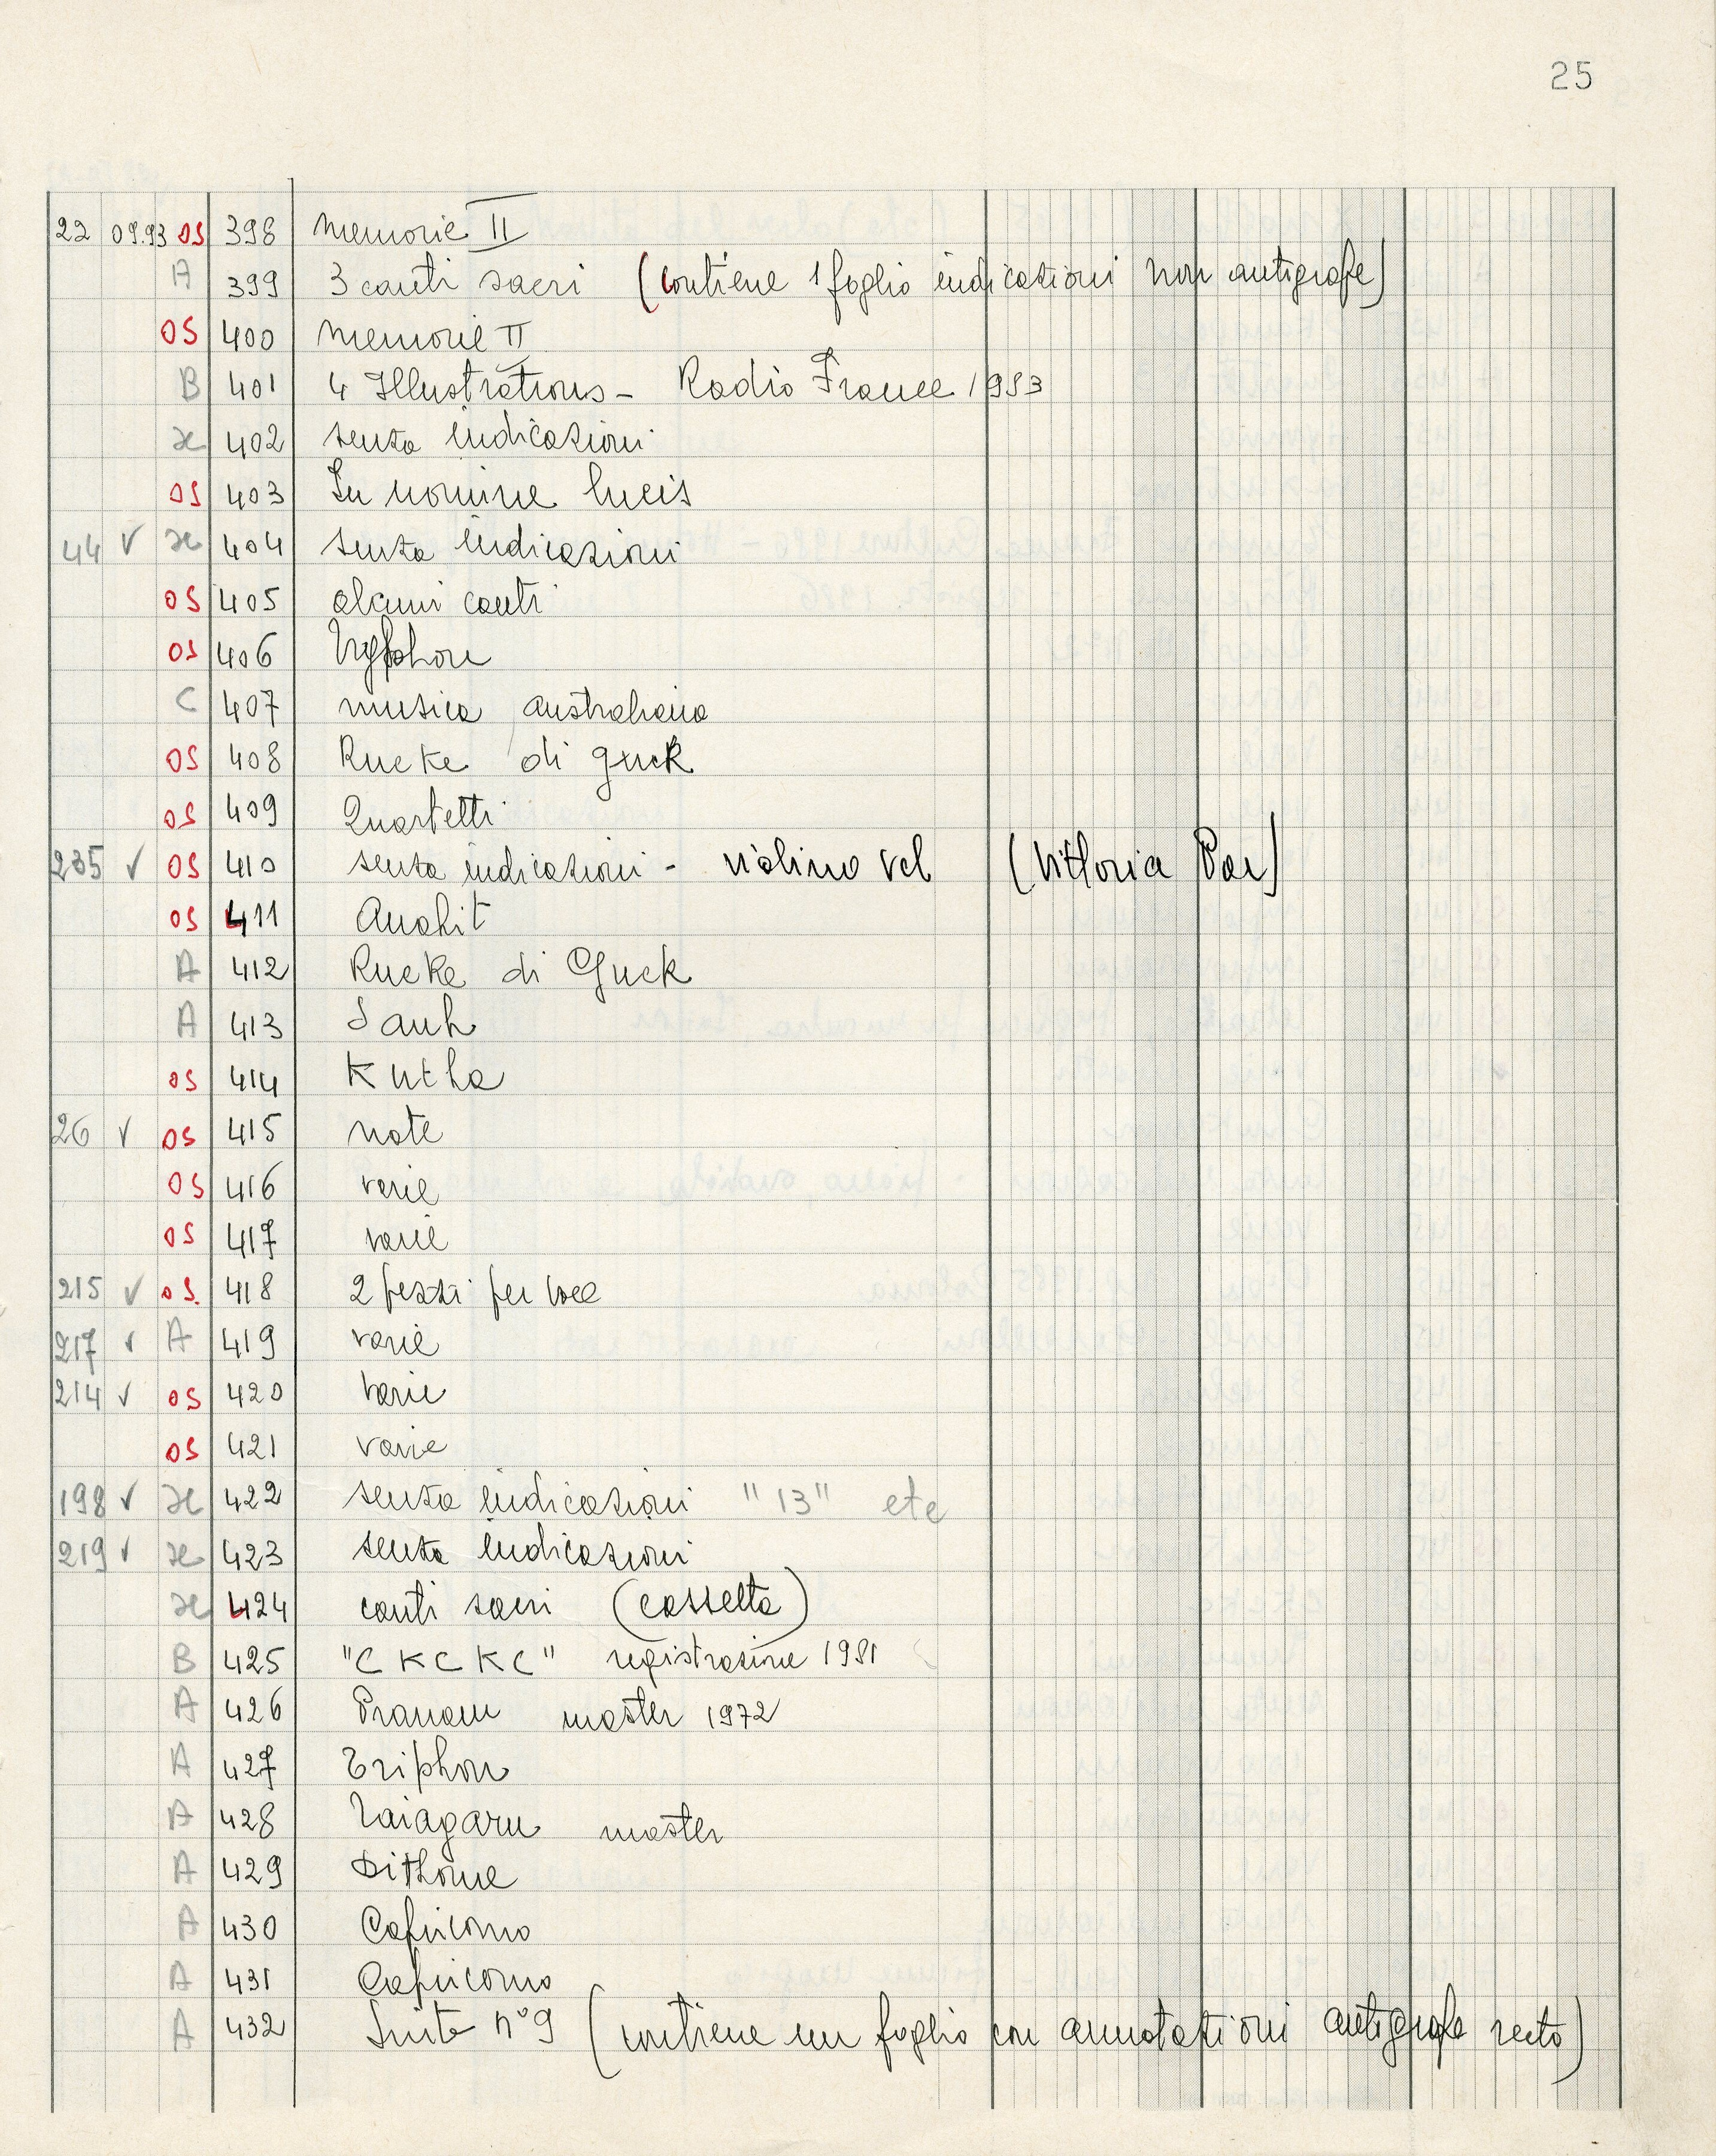
\includegraphics[width=0.3\textwidth]{docs/img/elenco_registro_Boido.jpg}
    \caption{Elenco registro Boido}
\end{wrapfigure}

C'è stata una primma catalogazione effettuata da \persona{Barbara Boido}{9999}{9999} subito dopo la morte di Scelsi che ad oggi è il secondo numero riportato nelle etichette dell'attuale catalogazione (NMGS<primo numero>-<secondo numero>).

Il primo tentativo sistematico di preservazione digitale risale al 1992, quando il Consiglio Direttivo della FIS ha commissionato a \personaViva{Frances-Marie Uitti}{1946} il trasferimento dei 278 nastri - come detto precedentemente di ''primaria importanza'' - su cassette DAT (Digital Audio Tape). 

Questa operazione, pur meritoria nelle intenzioni, presentava limiti significativi. Le cassette DAT, come osservato durante il laboratorio, soffrono di un degrado ''verticale'': diversamente dai nastri analogici, dove il deterioramento è graduale, i supporti digitali diventano completamente illeggibili superata una soglia critica di degrado.

Il progetto attuale di digitalizzazione, avviato nel 2006 in collaborazione con lo Studio Coltempo di Roma e proseguito dal 2007 con l'Istituto Centrale dei Beni Sonori e Audiovisivi (ICBSA)\cite{pro:beracpmm4ch2011}, sta per concludersi dopo oltre quindici anni di lavoro. Come emerso durante le sessioni di laboratorio, il numero effettivo di nastri di primaria importanza si è rivelato significativamente superiore alle stime iniziali: dai 178 nastri identificati da Frances-Marie Uitti nel 1992, si è passati a oltre 350 nastri contenenti materiale compositivo originale di Scelsi. Questa espansione del corpus è dovuta al ritrovamento di numerosi nastri di primaria importanza precedentemente classificati come secondari, confermando la natura parzialmente artificiosa della categorizzazione iniziale.

Lo stato di conservazione dei nastri presenta un quadro variegato. La maggior parte dei supporti si trova in condizioni accettabili, con un livello di rumore di fondo che, seppur presente, non compromette l'intelligibilità del contenuto sonoro. Tuttavia, circa il 2-3\% della collezione presenta patologie severe che richiedono interventi specialistici prima del trasferimento digitale.  Durante le sessioni di laboratorio, è stato possibile osservare direttamente il trattamento di alcuni di questi casi problematici, richiedendo la collaborazione con i tecnici specializzati della Discoteca di Stato per l'accesso alle attrezzature specifiche come i forni per il trattamento termico e gli aspiratori per la rimozione delle muffe.
\subsection{Tipologie di supporti e loro caratteristiche tecniche}
L'analisi dei supporti magnetici utilizzati da Scelsi rivela una storia tecnologica che attraversa quattro decenni. I nastri sono tutti da 1/4 di pollice di larghezza, registrati su macchine a due piste configurate per registrazione stereofonica o, più frequentemente, mono bidirezionale.

Le marche di nastro magnetico identificate durante il laboratorio includono:

\begin{enumerate}
    \item \textbf{Scotch}: I primi nastri utilizzati da Scelsi, rappresentano i supporti magnetici americani disponibili in Europa nel dopoguerra. Questi nastri hanno generalmente mantenuto buone caratteristiche di conservazione, con occasionali problemi di adesione tra le spire.
\end{enumerate}

\begin{enumerate}
    \item \textbf{Ampex}: Particolarmente problematici risultano i nastri Ampex 456, utilizzati negli studi professionali dagli anni Sessanta. Come documentato estensivamente durante le sessioni di laboratorio, questi nastri soffrono del fenomeno della ''sticky shed syndrome'': l'idrolisi del legante poliuretanico causa il distacco dello strato magnetico dal supporto.
\end{enumerate}

\begin{enumerate}
    \item \textbf{Agfa e BASF}: Nastri di produzione tedesca che presentano la caratteristica distintiva di riportare sulla costa del nastro non solo il nome del produttore ma anche il numero di matricola della partita di produzione. Questo dettaglio si è rivelato prezioso per la datazione dei materiali.
\end{enumerate}
\subsection{Friedrich Jaecker e l'identificazione dei contenuti}
Il musicologo \personaViva{Friedrich Jaecker}{1950} ha compilato un catalogo a partire dai primi 350-400 nastri identificando 174 frammenti.

Nel suo catalogo\cite{jaeckercatalogue}, Jaecker identifica con certezza materiali riconducibili a 54 opere di Scelsi distribuiti su 57 nastri. Questo dato, confrontato con i 189 manoscritti presenti nell'archivio cartaceo e i 117 titoli pubblicati, evidenzia la complessità del rapporto tra materiale registrato e produzione compositiva finale\cite[p. 47]{bernardini_pellegrini_scelsi_2016}.

L'analisi quantitativa del catalogo Jaecker rivela pattern significativi nella descrizione dei contenuti. Le occorrenze terminologiche mostrano: ''klavier/piano'' (114 menzioni), ''ondiola'' (111), ''improvvisazione'' (110), ''gestisch/gestuale'' (15) e ''ähnlich/simile a'' (14)\cite[p. 48]{bernardini_pellegrini_scelsi_2016}. Questa distribuzione lessicale riflette non solo la strumentazione prevalente nelle registrazioni, ma anche la natura processuale e comparativa del lavoro di identificazione.
\subsection{Metadati e informazioni periferiche}
Un aspetto critico emerso durante il laboratorio riguarda l'affidabilità delle informazioni riportate sulle scatole dei nastri. Scelsi utilizzava i contenitori come superficie di annotazione, registrando numeri di contatore, indicazioni per i trascrittori, frammenti di testo. Tuttavia, la pratica del compositore di riciclare sia nastri che contenitori rende queste annotazioni inaffidabili come fonte primaria di identificazione del contenuto.

Il database sviluppato per il progetto mantiene traccia di tutte le informazioni disponibili per ciascun nastro, includendo: numero d'ordine progressivo, produttore e tipo di nastro magnetico (come riportato sulla scatola), diametro delle flange, lunghezza misurata del nastro (in metri e piedi), materiale del nastro (acetato o poliestere), velocità di registrazione identificate, posizionamento audio (testa o coda), tipologia di registrazione, parametri tecnici del trasferimento digitale.

